\documentclass{elteikthesis}

\usepackage{tikz}
\usepackage{pgf-umlcd}
\usepackage{stuki}

\renewcommand{\umlfillcolor}{white}
\renewcommand{\umldrawcolor}{black}
\renewcommand{\umltextcolor}{black}

\usepackage{ucs}
\usepackage[utf8x]{inputenc}
\usepackage[english,hungarian]{babel}
\selectlanguage{hungarian}

\title{Függvény interpoláció megjelenítése}
\author{Szitár Gergő}
\supervisor{Dr. Krebsz Anna}
\supervisorstitle{egyetemi docens}
\period{Programtervező Informatikus BSc}
\thesisyear{2016}
\department{Numerikus Analízis tanszék}

\begin{document}

\frontmatter

	\maketitle
	\tableofcontents
	
\mainmatter

\chapter{Bevezetés}

\chapter{Felhasználói dokumentáció}
\section{Telepítés}
\section{Használat}
\section{Gyakran Ismételt Kérdések}

\chapter{Fejlesztői dokumentáció} 

\section{Osztály diagrammok}
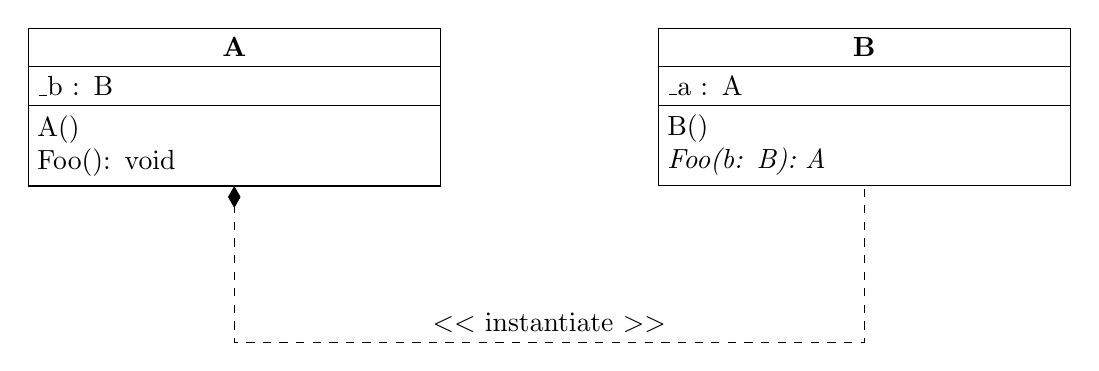
\begin{tikzpicture}
\begin{class}{A}{0,0}
	\attribute{\_b : B}
	\operation{A()}
	\operation{Foo(): void}
\end{class}

\begin{class}{B}{8 ,0}
	\attribute{\_a : A}
	\operation{B()}
	\operation [0]{Foo(b: B): A}
	
\end{class}

\draw[umlcd  style  dashed  line, diamond-]
	(A.south)
	|- (0, -4)
	-- node[above]{$<<$ instantiate $>>$}
	(8 ,-4)	-| 
	(B.south);

\end{tikzpicture}

\begin{stuki*}[6cm]{Valami}
  \stm{g}
  \stm*{sg, dg, g:}
  \stm*{x := }
  \begin{WHILE}{3}{\stm{sg}}
    \begin{IF}{1}{\stm*{\(dg.db < k  dg.db > m\)}}
      \stm*{x :  (dg.nev)}
    \ELSE
      \stm*{SKIP}
    \end{IF}
    \stm*{sg, dg, g:}
  \end{WHILE}
\end{stuki*}

\end{document}
